\documentclass{beamer}
\mode<presentation>
\usepackage{amsmath,amssymb,mathtools}
\usepackage{textcomp}
\usepackage{gensymb}
\usepackage{adjustbox}
\usepackage{subcaption}
\usepackage{enumitem}
\usepackage{multicol}
\usepackage{listings}
\usepackage{url}
\usepackage{graphicx} % <-- needed for images
\def\UrlBreaks{\do\/\do-}

\usetheme{Boadilla}
\usecolortheme{lily}
\setbeamertemplate{footline}{
  \leavevmode%
  \hbox{%
  \begin{beamercolorbox}[wd=\paperwidth,ht=2ex,dp=1ex,right]{author in head/foot}%
    \insertframenumber{} / \inserttotalframenumber\hspace*{2ex}
  \end{beamercolorbox}}%
  \vskip0pt%
}
\setbeamertemplate{navigation symbols}{}

\lstset{
  frame=single,
  breaklines=true,
  columns=fullflexible,
  basicstyle=\ttfamily\tiny   % tiny font so code fits
}

\numberwithin{equation}{section}

% ---- your macros ----
\providecommand{\nCr}[2]{\,^{#1}C_{#2}}
\providecommand{\nPr}[2]{\,^{#1}P_{#2}}
\providecommand{\mbf}{\mathbf}
\providecommand{\pr}[1]{\ensuremath{\Pr\left(#1\right)}}
\providecommand{\qfunc}[1]{\ensuremath{Q\left(#1\right)}}
\providecommand{\sbrak}[1]{\ensuremath{{}\left[#1\right]}}
\providecommand{\lsbrak}[1]{\ensuremath{{}\left[#1\right.}}
\providecommand{\rsbrak}[1]{\ensuremath{\left.#1\right]}}
\providecommand{\brak}[1]{\ensuremath{\left(#1\right)}}
\providecommand{\lbrak}[1]{\ensuremath{\left(#1\right.}}
\providecommand{\rbrak}[1]{\ensuremath{\left.#1\right)}}
\providecommand{\cbrak}[1]{\ensuremath{\left\{#1\right\}}}
\providecommand{\lcbrak}[1]{\ensuremath{\left\{#1\right.}}
\providecommand{\rcbrak}[1]{\ensuremath{\left.#1\right\}}}
\theoremstyle{remark}
\newtheorem{rem}{Remark}
\newcommand{\sgn}{\mathop{\mathrm{sgn}}}
\providecommand{\abs}[1]{\left\vert#1\right\vert}
\providecommand{\res}[1]{\Res\displaylimits_{#1}}
\providecommand{\norm}[1]{\lVert#1\rVert}
\providecommand{\mtx}[1]{\mathbf{#1}}
\providecommand{\mean}[1]{E\left[ #1 \right]}
\providecommand{\fourier}{\overset{\mathcal{F}}{ \rightleftharpoons}}
\providecommand{\system}{\overset{\mathcal{H}}{ \longleftrightarrow}}
\providecommand{\dec}[2]{\ensuremath{\overset{#1}{\underset{#2}{\gtrless}}}}
\newcommand{\myvec}[1]{\ensuremath{\begin{pmatrix}#1\end{pmatrix}}}
\let\vec\mathbf

\title{Matgeo Presentation - Problem 12.596}
\author{ee25btech11063 - Vejith}

\begin{document}


\frame{\titlepage}
\begin{frame}{Question}
Consider the system of linear equations:\\
\hspace*{6cm} $x-2y+3z=-1$,\\
\hspace*{6cm} $x-3y+4z= 1$,\\
\hspace*{6cm} $-2x+4y-6z= k$\\
The value of $k$ for which the system has infinitely many solutions is \underline{\hspace{2cm}} \hspace{5cm} \brak{\text{EC } 2015}\\
\end{frame}

\begin{frame}{Solution}
    Given equations are
\begin{align}
    \brak{1 \hspace{0.3cm} -2 \hspace{0.4cm} 3}\myvec{x\\y\\z}=-1\\
     \brak{1 \hspace{0.3cm} -3 \hspace{0.4cm} 4}\myvec{x\\y\\z}=1\\
      \brak{-2 \hspace{0.5cm} 4 \hspace{0.4cm} -6}\myvec{x\\y\\z}=k
\end{align}
These equations can be written in matrix form as
\begin{align}
    \begin{pmatrix}
        1 & -2 & 3\\
        1 & -3 & 4\\
        -2 & 4 & -6
    \end{pmatrix}\myvec{x\\y\\z}=\myvec{-1\\1\\k}
\end{align}
\end{frame}

\begin{frame}{Solution}
Forming the augmented matrix
\begin{align}
    \left(\begin{array}{ccc|c}
        1 & -2 & 3 & -1 \\
        1 & -3 & 4 & 1\\
        -2 & 4 & -6 & k\\
\end{array}\right) &\xleftrightarrow{R_2 \leftarrow R_2 -  R_1} \left(\begin{array}{ccc|c}
        1 & -2 & 3 & -1 \\
        0 & -1 & 1 & 2\\
        -2 & 4 & -6 & k\\
\end{array}\right)\\
&\xleftrightarrow{R_3 \leftarrow R_3 +  2R_1} \left(\begin{array}{ccc|c}
        1 & -2 & 3 & -1 \\
        0 & -1 & 1 & 2\\
        0 & 0 & 0 & k-2\\
\end{array}\right)
\end{align}
As in the augmented matrix the entries of third  row are 0 their linear combination should also give 0 
\begin{align}
    k-2=0\\
    \implies k=2
\end{align}
Now the system has 2 equations and 3 variables which has infinite solutions
\end{frame}

\begin{frame}{Plot}
    \begin{figure}[h!]
    \centering
    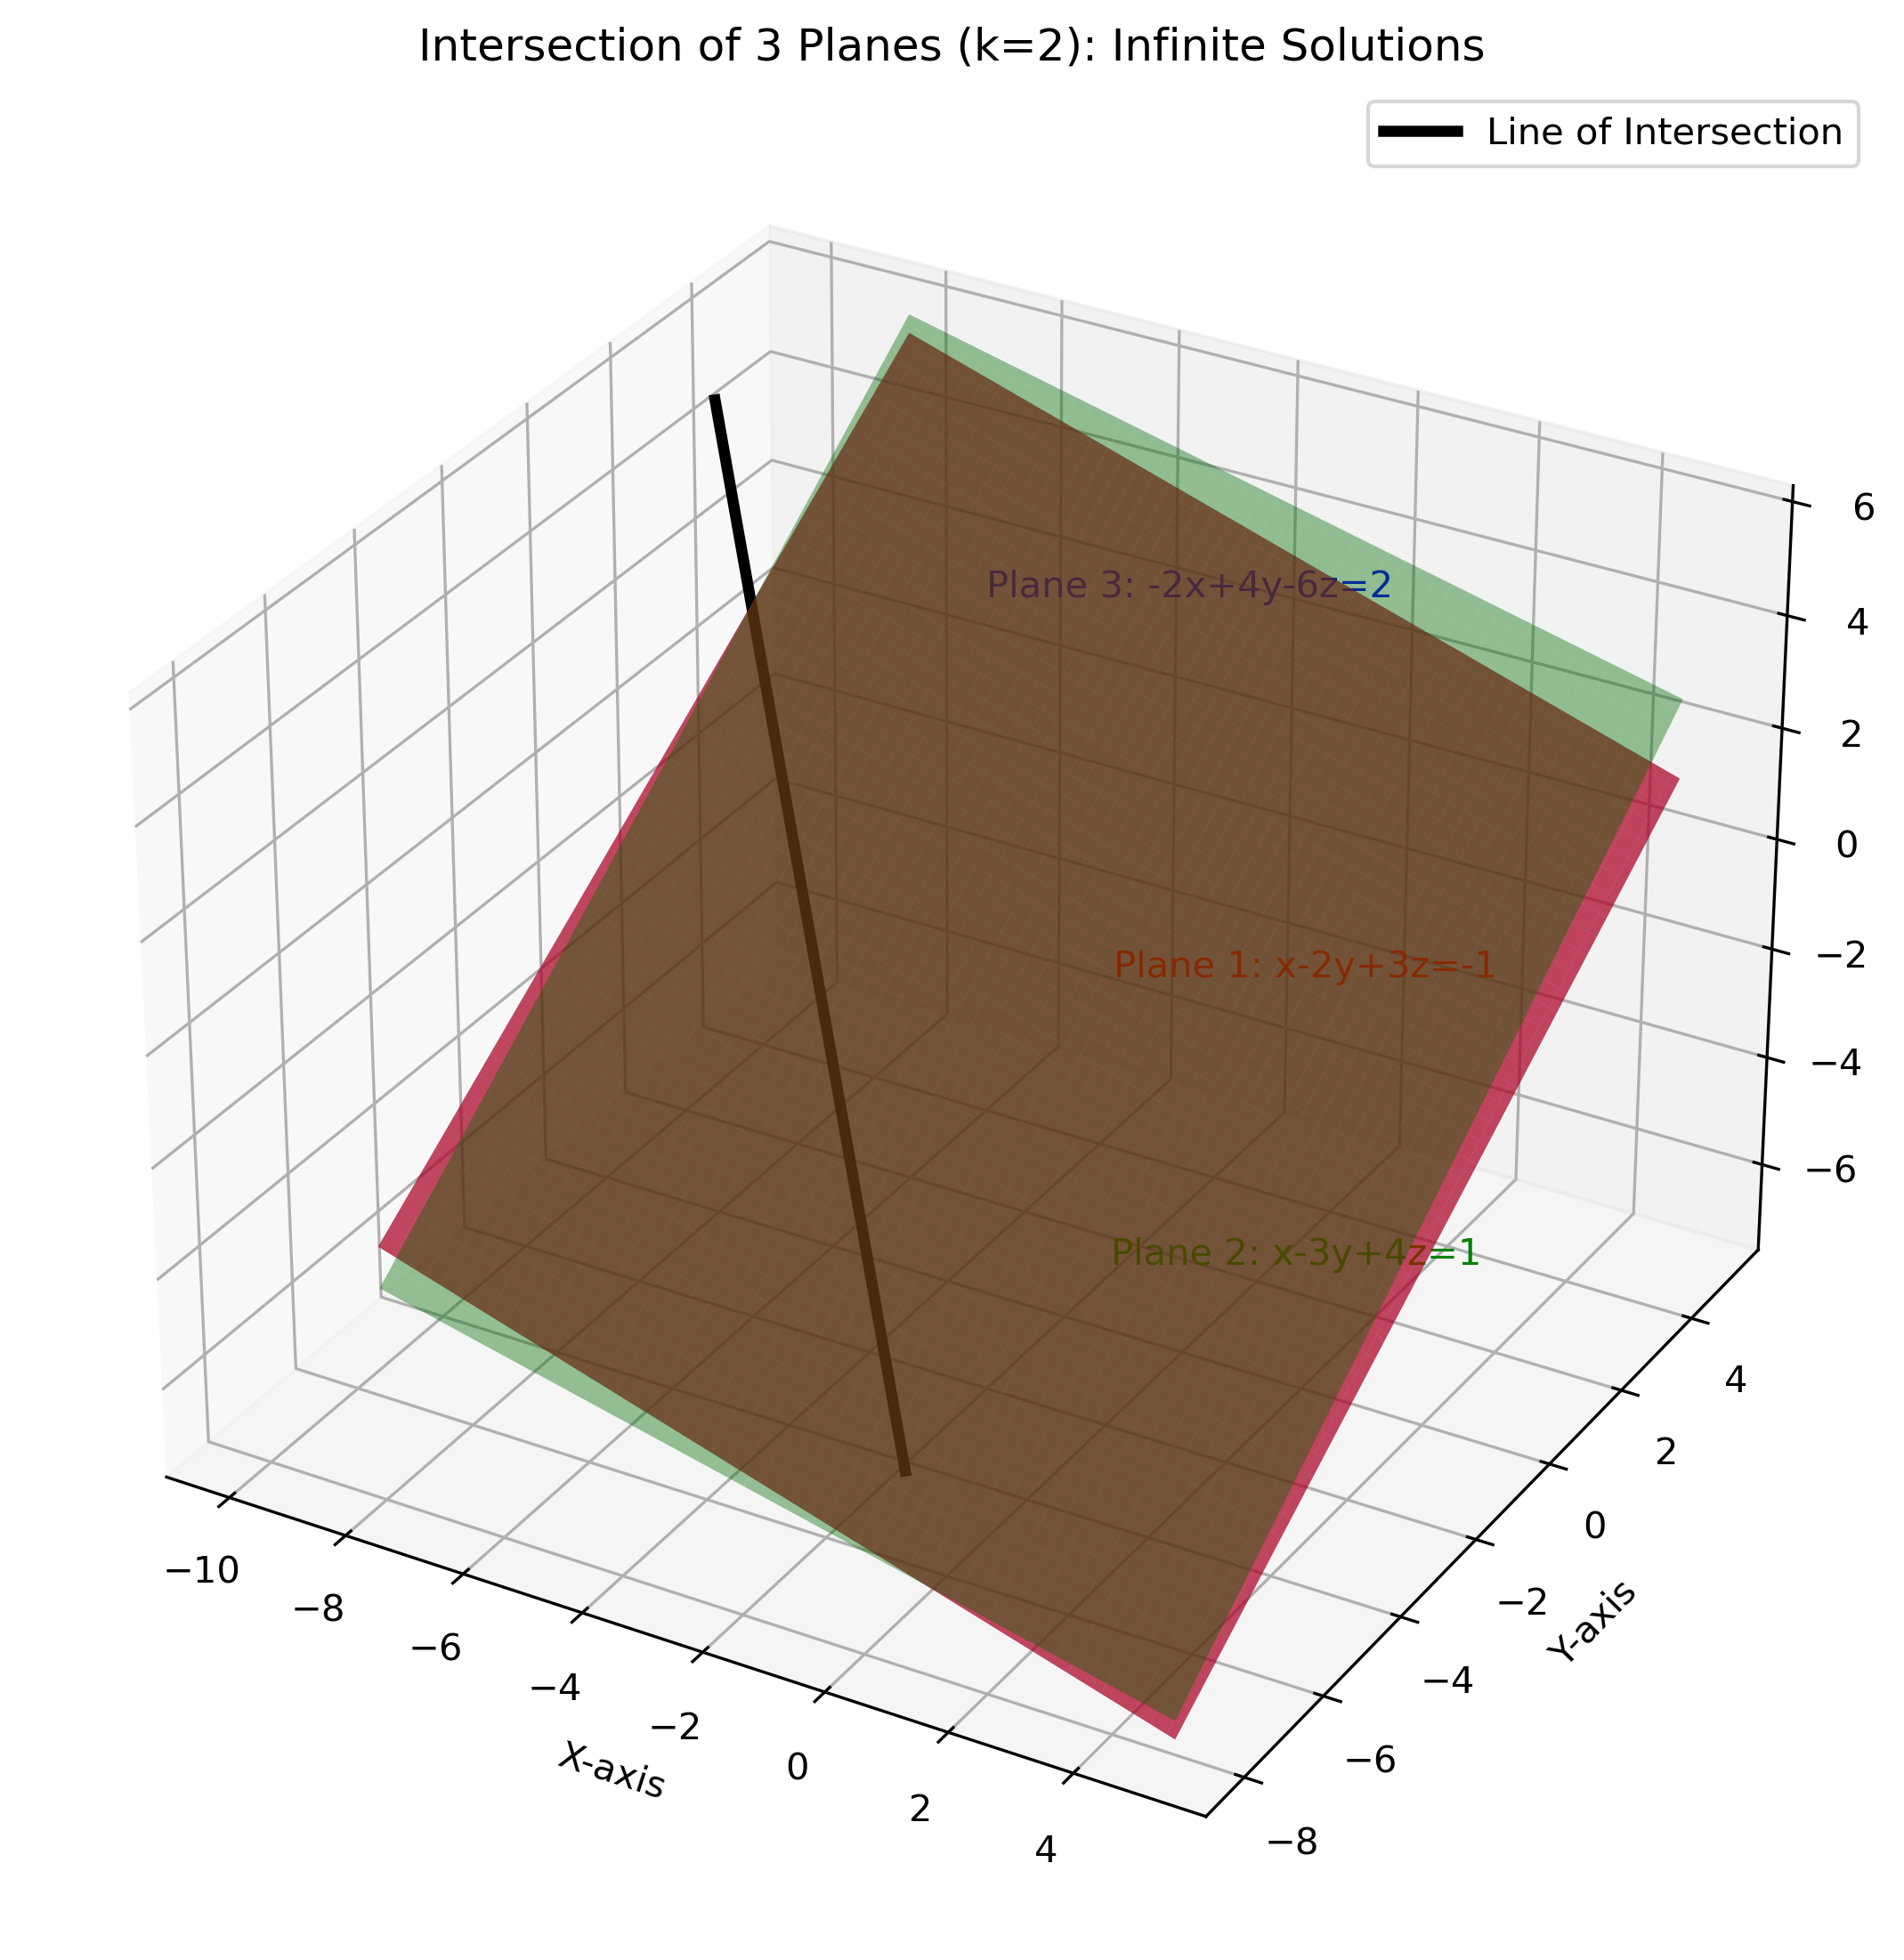
\includegraphics[width=0.7\columnwidth]{figs/01.png}
    \caption{}
    \label{fig:placeholder}
\end{figure}
\end{frame}

% --------- CODE APPENDIX ---------
\section*{Appendix: Code}

% C program
\begin{frame}[fragile]{C Code: Solution.c}
\begin{lstlisting}[language=C]
#include <stdio.h>

int main() {
    float mat[3][4] = {
        {1, -2, 3, -1},   // Equation 1
        {1, -3, 4, 1},    // Equation 2
        {-2, 4, -6, 0}    // Equation 3: RHS is k (we'll set this below)
    };

    float k;

    // Step 1: R2 = R2 - R1
    for (int i = 0; i < 4; i++) {
        mat[1][i] = mat[1][i] - mat[0][i];
    }

    // Step 2: R3 = R3 + 2*R1
    // RHS of R3 will be k, so we apply operation to it symbolically
    float rhs3 = k; // placeholder, we want to find the value of k

    // After row ops:
    // R3 = R3 + 2*R1
     k = 2;  // This satisfies the condition

    // Output the result to solution.dat
    FILE *fp = fopen("solution.dat", "w");
    if (fp == NULL) {
        printf("Error opening file.\n");
        return 1; }
    fprintf(fp, "The value of k for which the system has infinitely many solutions is: %.1f\n", k);
    fclose(fp);
  printf("The value of k is: %.1f (also written to solution.dat)\n", k);
    return 0;}
\end{lstlisting}
\end{frame}

% Python plotting
\begin{frame}[fragile]{Python: plot.py}
\begin{lstlisting}[language=Python]
import numpy as np
import matplotlib.pyplot as plt
from mpl_toolkits.mplot3d import Axes3D

# Define grid for planes
x = np.linspace(-8, 5, 100)
y = np.linspace(-8, 5, 100)
X, Y = np.meshgrid(x, y)

# Plane equations
Z1 = (-1 - X + 2*Y)/3          # Plane 1: x - 2y + 3z = -1
Z2 = (1 - X + 3*Y)/4           # Plane 2: x - 3y + 4z = 1
Z3 = (-2*X + 4*Y - 2)/6        # Plane 3: -2x + 4y - 6z = 2 (multiple of Plane 1)

# Plotting
fig = plt.figure(figsize=(12, 9))
ax = fig.add_subplot(111, projection='3d')

# Plot planes (red drawn last so it's visible on top of blue)
ax.plot_surface(X, Y, Z2, alpha=0.4, color='green')  # Plane 2
ax.plot_surface(X, Y, Z3, alpha=0.3, color='blue')   # Plane 3
ax.plot_surface(X, Y, Z1, alpha=0.6, color='red')    # Plane 1

# Line of intersection
t = np.linspace(-5, 5, 100)
x_line = -t - 5
y_line = t - 2
z_line = t
ax.plot(x_line, y_line, z_line, color='black', linewidth=3, label="Line of Intersection")
\end{lstlisting}
\end{frame}

\begin{frame}[fragile]{Python: plot.py}
\begin{lstlisting}[language=Python]
# Labels
ax.set_xlabel('X-axis')
ax.set_ylabel('Y-axis')
ax.set_zlabel('Z-axis')
ax.set_title("Intersection of 3 Planes (k=2): Infinite Solutions")

# Add plane labels
ax.text(2, -5, 3, "Plane 1: x-2y+3z=-1", color='red')
ax.text(2, -5, -2, "Plane 2: x-3y+4z=1", color='green')
ax.text(-6, 4, 2, "Plane 3: -2x+4y-6z=2", color='blue')

# Show legend
ax.legend()

# Save figure
plt.savefig("planes_intersection.png", dpi=300, bbox_inches='tight')

# Display figure
plt.show()

\end{lstlisting}
\end{frame}
\end{document}
